\section{Red neuronal simple}

Red neuronal simple, con una capa de entrada y una capa de salida de tipo softmax:
7.8\% de error sobre el conjunto de prueba y 5.6\% de error sobre el conjunto de
entrenamiento (tiempo de entrenamiento necesario: sobre un minuto usando una
implementación en un lenguaje interpretado como Matlab).

\subsection{Fundamentos teóricos}

tfhtfhtr

\subsection{Implementación}

\begin{figure}[H]
	\centering
	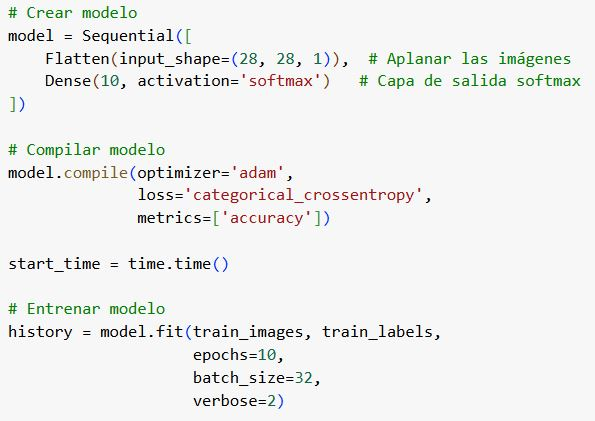
\includegraphics[width=0.7\textwidth]{imgs/model-red1.JPG}
	\caption{Modelado de la primera red neuronal simple}
	\label{fig:model-red1}
\end{figure}


\subsection{Análisis de resultados}

\begin{figure}[H]
	\centering
	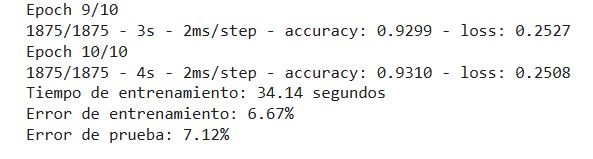
\includegraphics[width=0.7\textwidth]{imgs/results-red1.JPG}
	\caption{Resultados de la primera red neuronal simple}
	\label{fig:results-red1}
\end{figure}


\section{Red neuronal multicapa}

Red neuronal multicapa, con una capa oculta de 256 unidades logísticas y una capa
de salida de tipo softmax: 3.0\% de error sobre el conjunto de prueba y 0.0\% de error
sobre el conjunto de entrenamiento (tiempo de entrenamiento necesario: unos cuatro
minutos usando una implementación en un lenguaje interpretado como Matlab).

\subsection{Fundamentos teóricos}

\subsection{Implementación}

\begin{figure}[H]
	\centering
	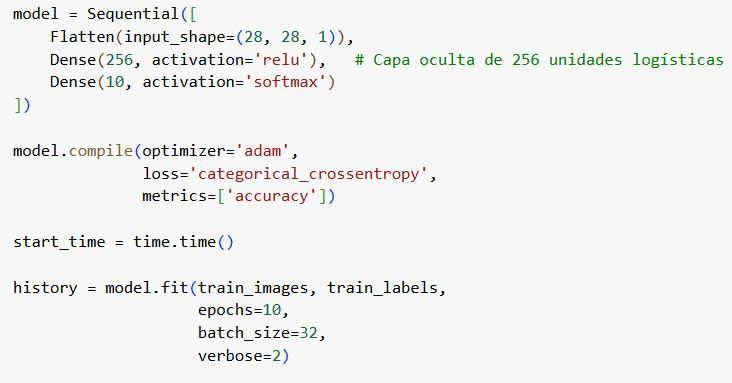
\includegraphics[width=0.7\textwidth]{imgs/model-red2.JPG}
	\caption{Modelado de la segunda red neuronal}
	\label{fig:model-red2}
\end{figure}

\subsection{Análisis de resultados}

\begin{figure}[H]
	\centering
	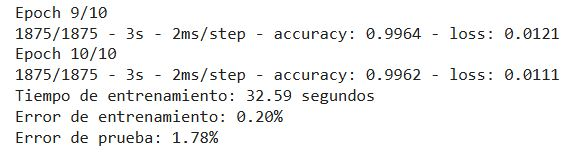
\includegraphics[width=0.7\textwidth]{imgs/results-red2.JPG}
	\caption{Resultados de la segunda red neuronal}
	\label{fig:results-red2}
\end{figure}


\section{Red neuronal convolutiva}

Red neuronal convolutiva entrenada con gradiente descendente estocástico: 2.7\%
de error sobre el conjunto de prueba (tiempo de entrenamiento necesario: unos 13
minutos usando una implementación en un lenguaje interpretado como Matlab).

\subsection{Fundamentos teóricos}

\subsection{Implementación}

\begin{figure}[H]
	\centering
	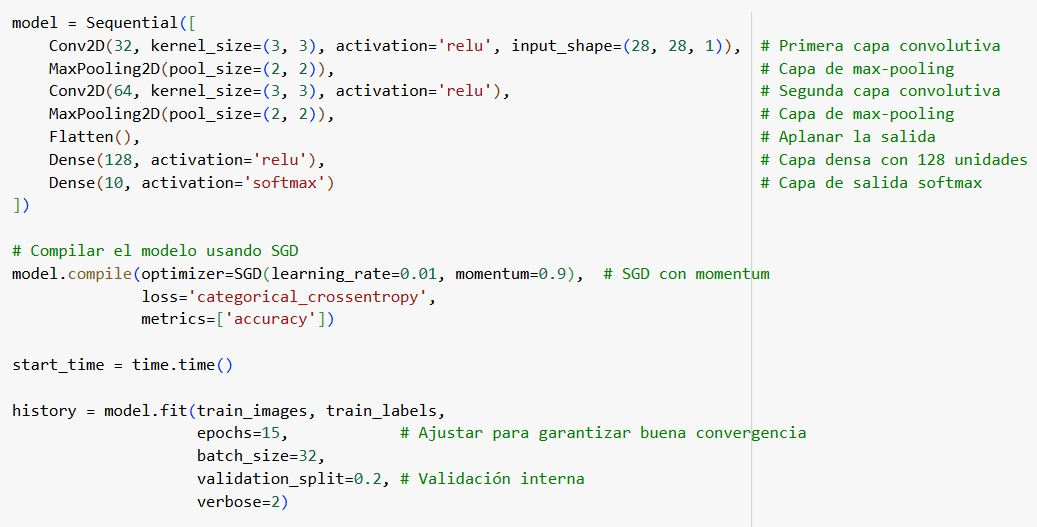
\includegraphics[width=0.7\textwidth]{imgs/model-red3.JPG}
	\caption{Modelado de la tercera red neuronal}
	\label{fig:model-red3}
\end{figure}

\subsection{Análisis de resultados}



\section{Deep learning}

\textit{Deep learning} usando pre-entrenamiento de autoencoders para extraer características de las imágenes usando técnicas no supervisadas y una red neuronal simple con una capa de tipo softmax: del 1.8\% al 2.2\% de error sobre el conjunto de prueba (tiempo de entrenamiento necesario: unos veinte minutos usando una implementación en un lenguaje interpretado como Matlab).

\subsection{Fundamentos teóricos}

\subsection{Implementación}

\begin{figure}[H]
	\centering
	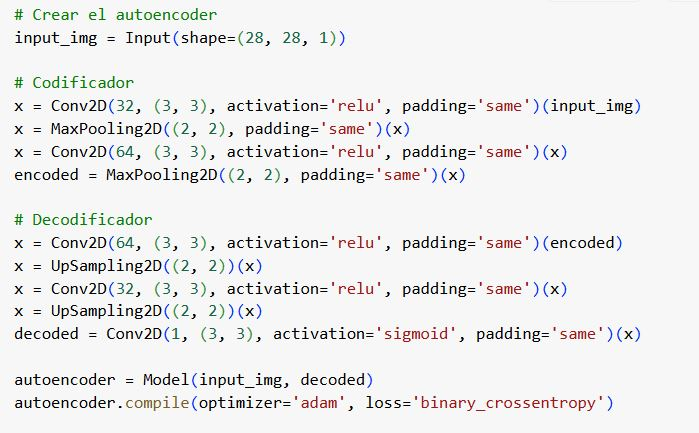
\includegraphics[width=0.7\textwidth]{imgs/model-1-red4.JPG}
	\caption{Modelado de la cuarta red neuronal}
	\label{fig:model-1-red4}
\end{figure}

\begin{figure}[H]
	\centering
	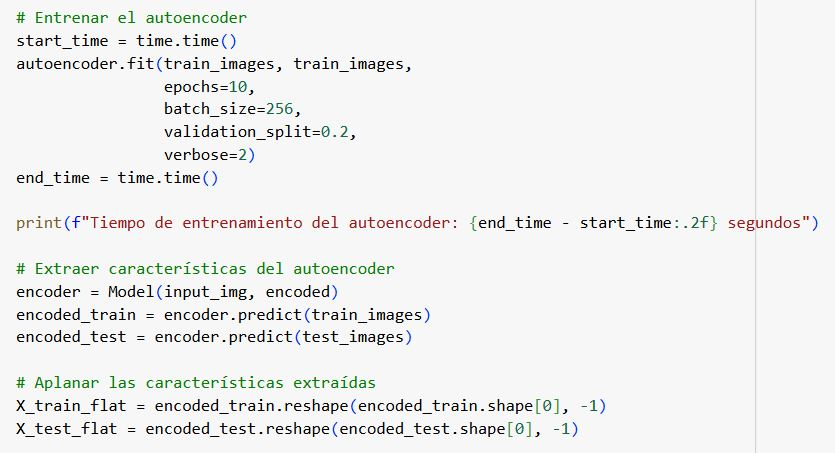
\includegraphics[width=0.7\textwidth]{imgs/model-2-red4.JPG}
	\caption{Modelado de la cuarta red neuronal}
	\label{fig:model-2-red4}
\end{figure}

\begin{figure}[H]
	\centering
	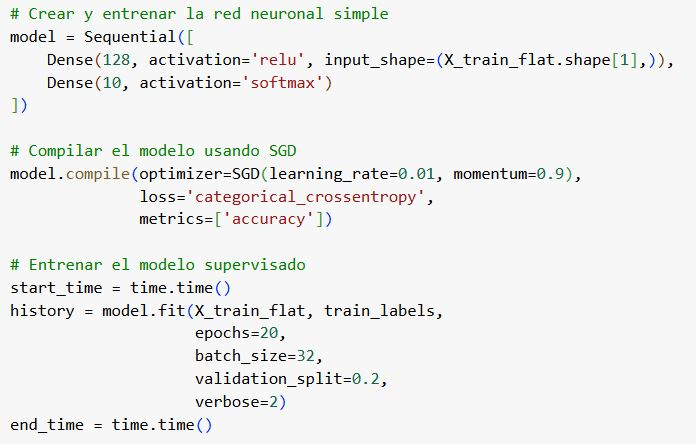
\includegraphics[width=0.7\textwidth]{imgs/model-3-red4.JPG}
	\caption{Modelado de la cuarta red neuronal}
	\label{fig:model-3-red4}
\end{figure}


\subsection{Análisis de resultados}

\begin{figure}[H]
	\centering
	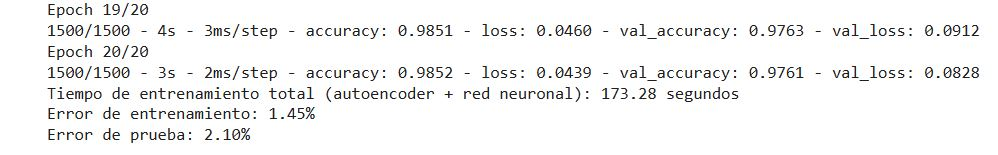
\includegraphics[width=0.7\textwidth]{imgs/results-red4.JPG}
	\caption{Resultados de la cuarta red neuronal}
	\label{fig:results-red4}
\end{figure}



\section{Red neuronal combinada mejorada}

Llegar a 99.7\% mínimo 98

\subsection{Fundamentos teóricos}

\subsection{Implementación}

\begin{enumerate}
	\item Dividir train set en validation set
	\item Data augmentation
	\item Convolutiva
	\item EarlyStopping
	\item ReduceLROnPlateau
\end{enumerate}


\subsection{Análisis de resultados}


